\subsection{Módulo genérico de los cambios de vías simples}
	\label{sec:ACG_ssw}
	
	El módulo \textit{SingleSwitches} es el encargado de implementar el funcionamiento de los cambios de vías simples en la red ferroviaria. El ACG utiliza la información otorgada por el RNA para determinar cuales son los \textit{netElements} conectados mediante el cambio de vías, los \textit{netElements} más próximos. Esta información se utiliza para implementar las entradas del módulo \textit{SingleSwitches} donde se reporta el estado de ocupación de los \textit{netElements} (\textit{ocupation}). Además, se implementan las conexiones de indicación, comando y correspondencia para poder leer, escribir y reportar el estado del cambio de vías, respectivamente. Finalmente, el ACG implementa las conexiones a todas las rutas que buscarán controlar el cambio de vías y todo los mecanismos para obedecer solo a una de ellas, de cumplirse las condiciones. El diagrama de bloques de las máquinas de estado finitas con camino de datos diseñado para lograr este objetivo se muestra en la Figura \ref{fig:SSW_module}.
	
	\begin{figure}[H]
		\centering
		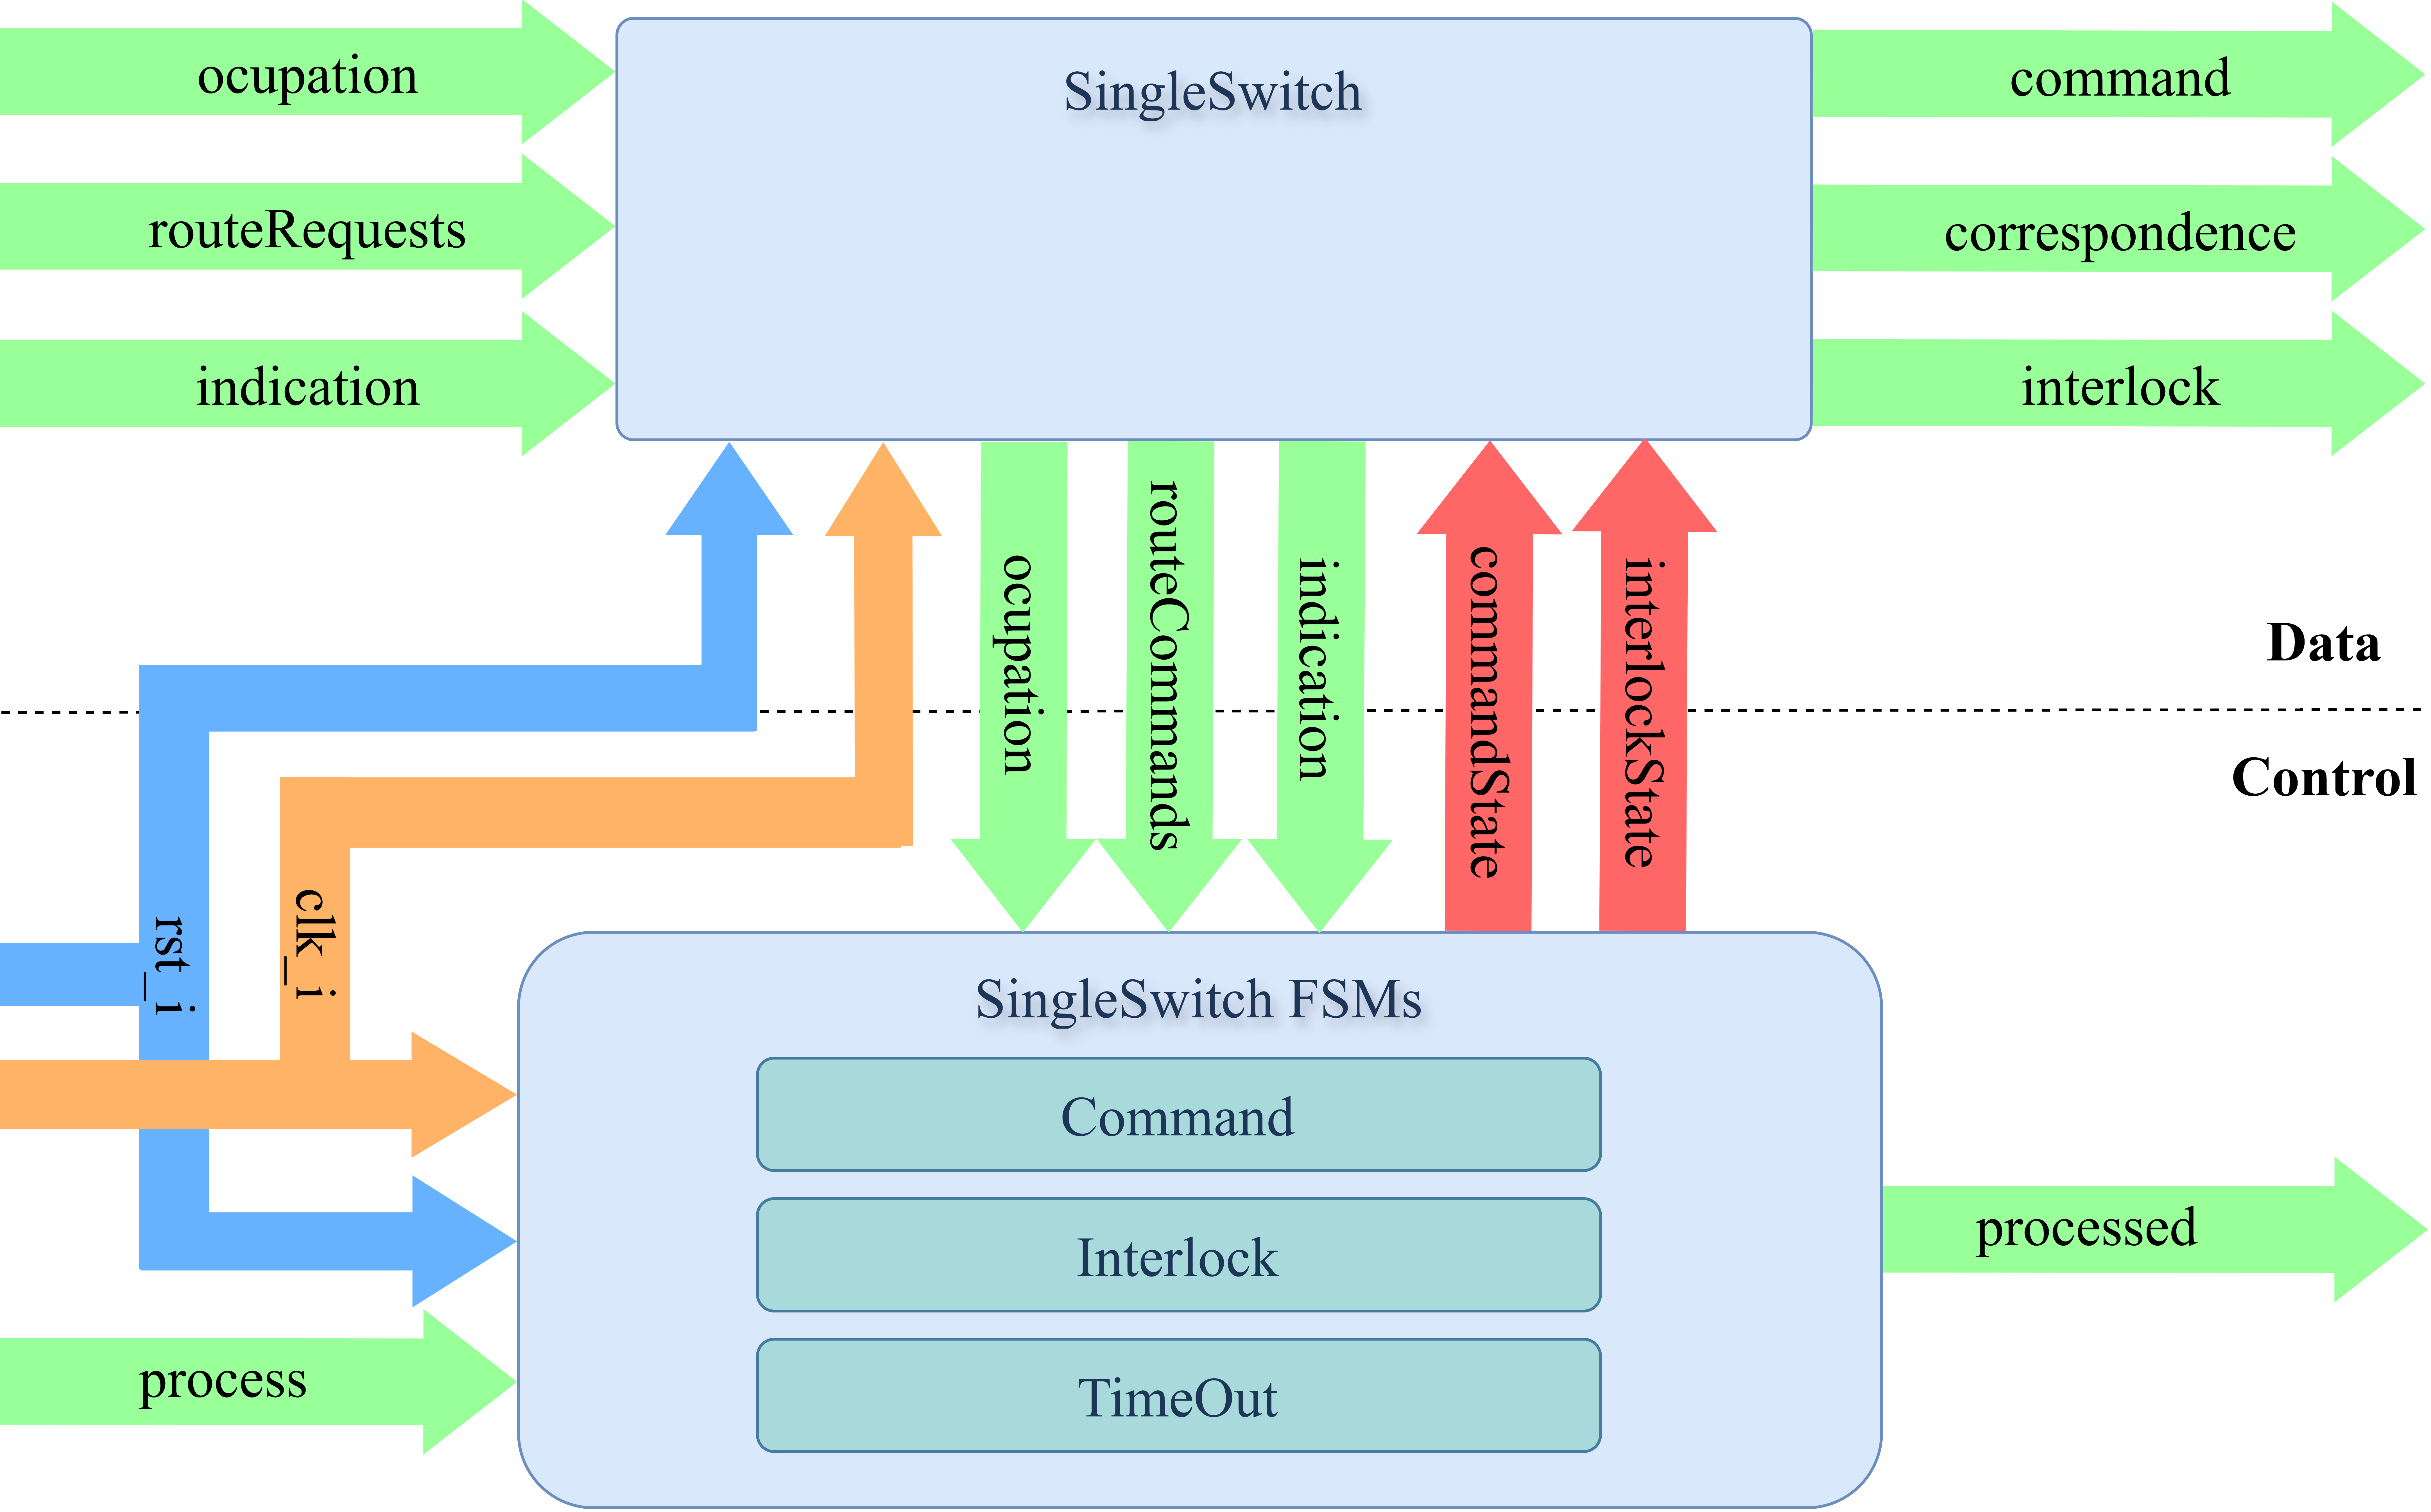
\includegraphics[width=1\textwidth]{Figuras/SSW_module}
		\centering\caption{FSMD del módulo genérico de \textit{SingleSwitches}.}
		\label{fig:SSW_module}
	\end{figure}
	
	Como fue explicado en la Sección \ref{sec:switches}, un cambio de vías simple puede adoptar dos posiciones: normal y reversa. Adicionalmente, es necesario contemplar que mientras la indicación no reporte una posición definida, normal o reverse, se deberá asumir que el cambio de vías se encuentra en transición de un estado al otro. Dicha transición debe ser corta, ya que de no completarse el movimiento puede ser tanto que el cambio de vías se encuentra atascado cómo que el comando o la indicación se encuentren desconectados del actuador. Esta funcionalidad, junto con el comportamiento del cambio de vías genérico se define en la red de Petri de la Figura \ref{fig:SSW_Petri}.
	
	\begin{figure}[H]
		\centering
		\includegraphics[width=1\textwidth]{Figuras/SSW_Petri}
		\centering\caption{Red de Petri del modelo dinámico de \textit{SingleSwitches}.}
		\label{fig:SSW_Petri}
	\end{figure}
	
	Un cambio de vías en estado reversa iniciará su transición si alguna de las rutas envía un comando para modificar la posición a normal, siempre que el cambio de vías no se encuentre enclavado por otra ruta que lo esté utilizando. Durante la transición, salvo que ocurra un timeout, el cambio de vías pasará al estado normal si se confirma la indicación normal y no el comando normal no fue cancelado por la ruta. Análogamente, el cambio de vías puede pasar del estado normal al reversa mediante la secuencia opuesta. Debiendo cumplir las mismas condiciones de no estar enclavado antes de mover el cambio de vías, confirmación de indicación y comando, y realizar todo el proceso dentro de un tiempo determinado.
	
	En el caso del timeout, se considera que si el cambio de vías no reporta una posición final en menos de un tiempo determinado, entonces el cambio de vías debe volver al estado anterior, de ser posible. De lograrse este o no, el cambio de vías igualmente quedará anulado y no podrá ser utilizado por la ruta que lo demanda, prohibiendo la habilitación de dicha ruta.
